\section{Evaluation of the Project}
Testing and evaluation were vital parts of the project, to ensure that the system produced, both contained all the functionality it should have, it adhered to all the constraints place upon it and that it was actually usable. Three stages of testing were therefore conducted. The first of these was functionality testing, in which the functional requirements of the system would be evaluated, and the system would be testing to see whether or not it implements this functionality. The next stage was non-functional testing, in which the non-functional requirements would be evaluated in turn, to ensure the system abided by them. The final stage was user feedback testing, in which a group of participants would actually be using the system. In this stage, three systems would be evaluated: MATLAB, FuzzyToolkitUoN, and this project; in order to determine which provided a better user experience.

\subsection{Functional Testing}
In this section, each of the functional requirements laid out in section \ref{sec:funcs} have been evaluated in turn, to ensure the system meets them. Knowledge of the inner workings of the system is not actually necessary to understand these tests, as they simply check whether functionality is present, and are not concerned as to how the system actually implements it (this is known as black box testing \cite{beizer1995black}). A complete listing of all the tests conducted, and their results, can be found in appendix \ref{app-ctl}.

\subsection{Non-Functional Testing}
In this section, each of the non-functional requirement laid out in section \ref{sec:non-funcs} have been enumerated, and the success to which they have been achieved has been detailed. The purpose of this is to evaluate how well the system has adhered to the constraints placed upon it.

\paragraph{Accessibility}\ \\
This was one of the biggest goals for the system, as it was one of it's main reasons for conception. The problem with most fuzzy logic software systems currently is that they are difficult to use, or difficult to access. That is why the project proposed in this report has accessibility improvements as one of it's main goals. To accomplish this, the system is entirely web based. The advantage of this, is that the user can access the system from any computer, running any operating system. This cross compatibility greater improves the outreach of the software, as no users will be unable to use it. Further to this, the system front end is constructed entirely in HTML, CSS, and JavaScript. This means that the user does not require the download of any additional software, or applications, to use this system (which would not be case if Adobe Flash, or Java had been used). 

\paragraph{Usability and Operability}\ \\
This is a goal of the system that is difficult to quantitatively measure. In order to actually test this goal, a set of participants of varying skill levels were asked to complete a list of tasks, using this system, and compare this to doing the same tasks in similar systems. The detailed results of these tests can be found in section \ref{sec:uft}. After the user feedback testing, it was found that the majority of participants preferred this new system, over the other two that were tested (MATLAB's fuzzy toolbox, and FuzzyToolkitUoN). The major reasons for this were the ``waterfall'' style to task complete (each task was laid out in a logical manner, and followed on smoothly from the last), and the clean, uncluttered user interface. 

\paragraph{Maintainability}\ \\
To aid with the eventual goal of the system back end being interchangeable with any back end that can process fuzzy logic, the system needed to be coded so that is was easily maintainable, and easily expandable. In order to achieve this, the code has been written in a modular fashion, split across multiple files. Each file deals with exactly one action (file manipulation, rule creation, evaluation, etc.), and thus adding new functionality should be relatively easy. Each function has been listed with the purpose of it, the parameters it takes (and their types), and the value it returns, if any. This means identifying the purpose of functions it extremely simple, and any maintainer will easily be able to interpret how the system functions. 

\paragraph{Quality}\ \\
To ensure that this system reflects well both on myself, and the University of Nottingham, it was made to be of the highest quality possible. The system has been built with a vast quantity of error handling methods, so that the system should not crash under operation, and should function exactly as the user expects. Helpful, and positive, error messages accompany any error handling methods, so the user can rectify any mistakes they make. 

\paragraph{Resource Requirements and Constraints}\ \\
As the system is a aimed at any level of user, no assumptions as to the level of hardware they may possess can be made. This means that the system must be built to be as light weight as possible, as to not overwhelm the user's device. Fortunately, the technologies used to build the front end (CSS, HTML and JavaScript) are relatively light weight, and the front end has minimal processing requirements. The main processing that takes place is on the server side, when the inference process takes place.

\paragraph{Cross Platform Compatibility}\ \\
As mentioned previously, the system is built with entire cross compatible languages, and only requires the user have an internet connection, and a web browser installed. Aside from these, there are no compatibility issues the system presents, as it is entirely web based, and requires no additional resources to function. There is potential that the system would not work on extremely old operating systems, but all operating systems that are currently being supported by their develop should function correctly.

\paragraph{Security}\ \\
In a web based system, there is potential for many security issues to be present. However, in this system, that is not the case, as it does not store any user data, and the only information stored on the user's computer, are the fuzzy systems that they create. To give the user's peace of mind when downloading their files, the contents of it are displayed to them, before they are able to press the download button. No cookies are stored on the user's computer, so this is not a security concern (although this may have improved the user experience, as detailed in section \ref{sec:mui}).


\paragraph{Reliability and Robustness}\ \\
As the system will be used by both expert users, and novices, it is important that it is as robust as possible. For this, extensive error trapping has been implemented throughout the system, so that any incorrect values entered by the user are dealt with accordingly, and do not cause the system to crash. The reliability and robustness of the system are important so that the expert users are not inhibited whilst working, and novices users are not left confused (as they would not be able to tell the difference between a mistake they have made, and the system crashing). Testing of the system was carried out by both novice users, and expert users, to identify any bugs in the system, and any usability issues, details of which can be found in section \ref{sec:uft}.

\paragraph{Documentation}\ \\
Large software documentation manuals are an extremely unintuitive way to find information on a software system. This fact stands even truer when looking at the novice audience, as a large documentation manual would simply be too daunting for them, and discourage them from using the system if they got stuck. To combat this, the system presented in this report does not have an external documentation. Instead, documentation is present in the system in the form of a help button being on each page. When clicked, a pop-up will be displayed, giving details on the workings of that specific page. This short explanation of how the page works is much more useful to the user, as it is concise, and easily locatable (always in the top right hand corner of the segment they are on, and always green). As far as documentation of the code, as has been mentioned, JavaDoc style comments will accompany every function written, that will describe what the function does, what parameters it takes (and their type), and what that function returns (if anything). 

\paragraph{Disaster Recovery}\ \\
During the lifetime of the project, the source code was stored in a private GitHub repository. This meant that the loss of code was not an issue, as it was backed up securely on the GitHub servers. As far as the system itself, due to the extensive error trapping that was present, the system was relatively robust, and would not crash due to user input. The only issue that remained, was if the user closed the system before saving their work. Unfortunately, this was not an issue that could be resolved without the implementation of cookies, that would have then raised a security concern. There was an attempt to include a pop-up, so that when the system was closed, the user was warned, but this was not implemented successfully. 

\subsection{User Feedback Testing}
\vspace{-2mm}
\label{sec:uft}
An important part of evaluating the usability and accessibility of the produced system was to have real world users attempt to actually use it \cite{nielsen1992usability}. In order to do this, several sessions were set up, and participants of various skills levels, both in terms of computers, and fuzzy logic, were invited along to complete a list of tasks using the software produced. So that comparative comments could be made, these same participants were also asked to complete the same list of tasks in two other similar software systems: FuzzyToolkitUoN, and MATLAB's fuzzy toolbox. After each task, the users would be asked for their feedback and opinions on the system, and how they felt it compared to the other systems.\ \\
\ \\
There were a total of 23 participants in these studies, split into four main categories, based on their skill level in fuzzy logic, and using computers in general. These groups will be referred to throughout this section, and the table in figure \ref{fig:skill-table} summarises the characteristics of the participants of each group. 

\begin{figure}[ht!]
\begin{center}
\begin{tabular}{cccc}
\hline
\textbf{Group} 	& \textbf{\# of Members} & \textbf{Fuzzy Logic Skill} & \textbf{Computer Skill} \\
\hline
1				& 7 						 & Low			& Low		\\	
2				& 5  						 & Low			& High		\\
3				& 3 						 & High			& Low 		\\
4				& 8 						 & High 		& High		\\
\hline
\end{tabular}
\end{center}
\captionsetup{justification=centering,margin=2cm}
\vspace{-4mm}
\caption{Number of members in each group of the study, with their accompanying skill levels}
\label{fig:skill-table}
\vspace{-2mm}
\end{figure}
\noindent 
Along with the user experience feedback that was recorded in these studies, the time taken for the user to complete the task list in each of the software systems, along with their favourite and least favourite systems was also recorded. The full results for this can be found in appendix \ref{app-torous}, and will be referred to throughout this section.\ \\
\ \\
The tasks were designed to evaluate as many of the cross-compatible features of the systems, so that they could be compared. The task itself was to implement the fuzzy tipper example, that is a popular first system for those learning fuzzy logic. The list of instructions given to the users can be found in appendix \ref{app-userEval}.

\subsubsection{Evaluation of FuzzyToolkitUoN}
% The exact setup (R console w/o ftu installed)

% Confusion between the R interface and console (assumed most functionality would be in the R gui interface)
% Attempt to use the inbuilt R help, to no avail
% Most interaction (especially with those of low skill level) was copy+paste from the example in the docs, and modifying for their needs
% variable assignment confusion throughout
% ``This is confusion'' Helplessness
% After multiple additions of mfs, most users began to understand what was expected
% Bam, rules; wide spread confusion <- many rules were wrong and thus system did not work
% mistakes were nigh-on impossible to resolve for novice users, intervention necessary
% poor understanding of evaluation across all groups
% treating the FIS as an object and indexing into it, confusing 
% some vital examples in the docs aren't sufficient 
% terrible error messages, mostly R garbage

\subsubsection{Evaluation of MATLAB Fuzzy Toolbox} 	
% far too much on the screen at once, very confusing
% so many windows open! confusion as to wheter to close them or keep them
% some boxes look like they should be editable, but aren't
% better than FTU atleast
% rectifying mistakes was must simpler
% menu system confusing and cumbersome
% no errors, would just attempt to fix your problems for you -> confusing

\subsubsection{Evaluation of My Project}	
% water fall flow
% clean interface, bootstrap is nice
% graphs are nice, more colourful than MATLAB 
% rule ui is super intuitive
% very easy to use
% much quicker (tab for speed)
% errors were friendly

\subsubsection{Summary of Evaluations}	
The main two factors that were observed whilst the participants were completing the tasks were the speed at which they could do so, and the ease. Generally a faster completion time meant either a high level of understanding, or an easier piece of software to use. The graph in figure \ref{fig:times} shows a bar chart representing the average time taken for each group to complete the task list, in each software system, as well as the average for all participants. The data collected clearly indicates that using FuzzyToolkitUoN to complete the tasks was the most difficult (taking on average  35 minutes), which, after speaking to the participants, was a result of it's poor user interface, steep learning curve, and reliance on checking a huge documentation manual. Both of the graphical user interface systems faired much better, with MATLAB being the second fastest to use (with an average time of 18 minutes), and the software system proposed in this report taking on average 10 minutes (an improvement of 44\% on MATLAB, and 71\% on FuzzyToolkitUoN). 
			
\begin{figure}[ht!]
	\begin{center}
		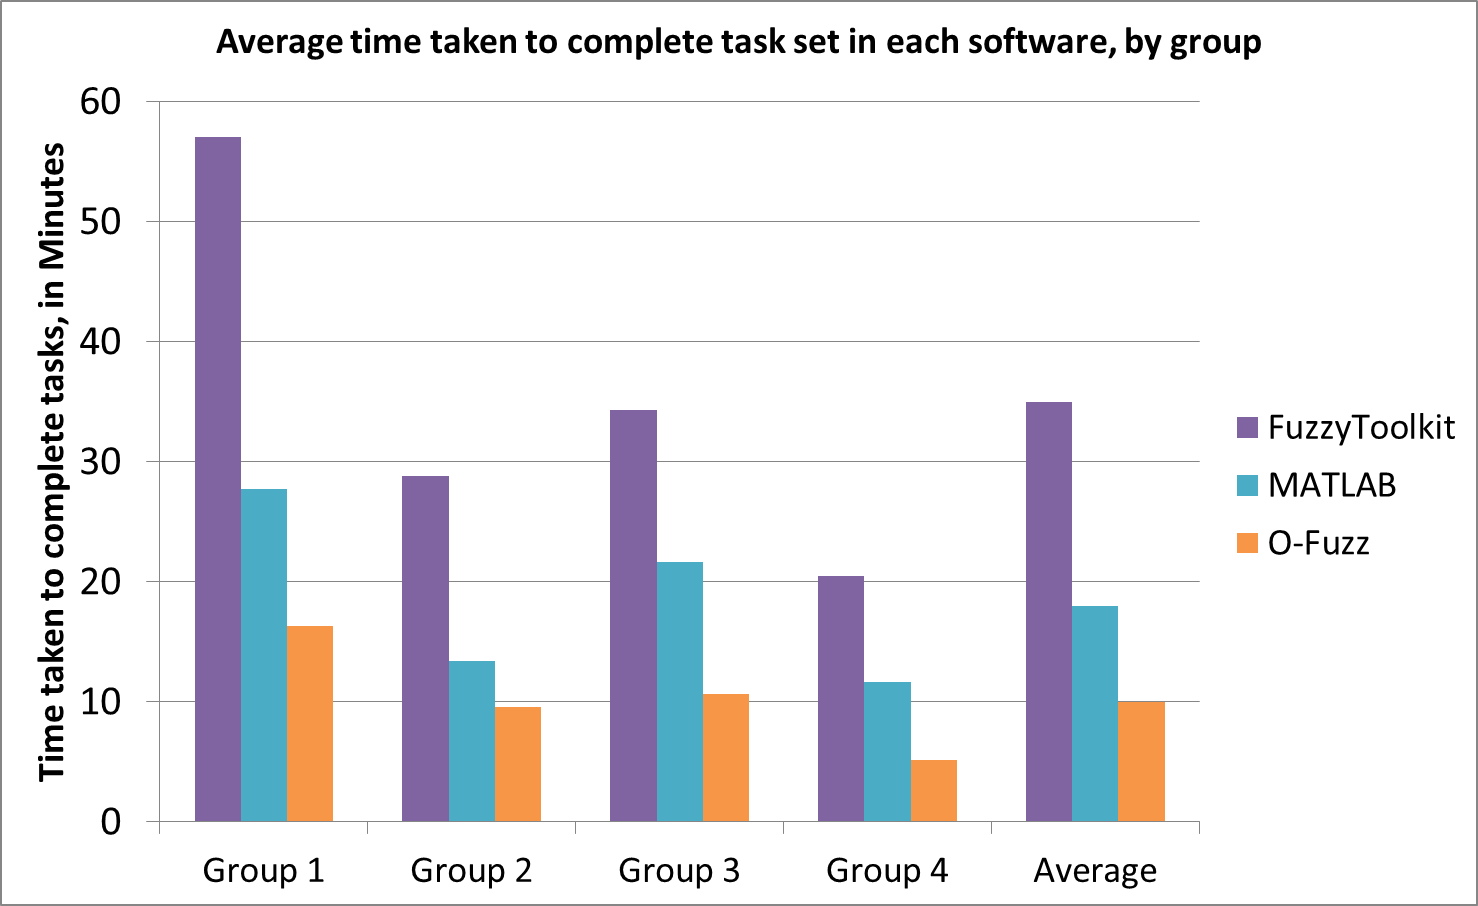
\includegraphics[width=0.9\textwidth]{images/timeTaken}
	\end{center}
	\vspace{-5mm}
	\captionsetup{justification=centering,margin=2cm}
	\caption{Bar chart of average time taken to complete the task set in the different software systems, by group}
	\label{fig:times}
	\vspace{-2mm}
\end{figure}
\noindent 						
Whilst the time taken to complete the tasks was a strong indicator of the success of the software system, it was also important to ask the participants which system they \emph{enjoyed} using the most. The results for this were conclusive, with 95.7\% of participants (across all categories) claiming FuzzyToolkitUoN was the piece of software they enjoyed using the least. The main reasons for this were the command line interface being difficult to use, visualisation of the system itself being unintuitive, there was a necessity to constantly refer to the large documentation manual, and that it was conceptually confusing for many computer novices. 

\begin{figure}[ht!]
	\begin{center}
		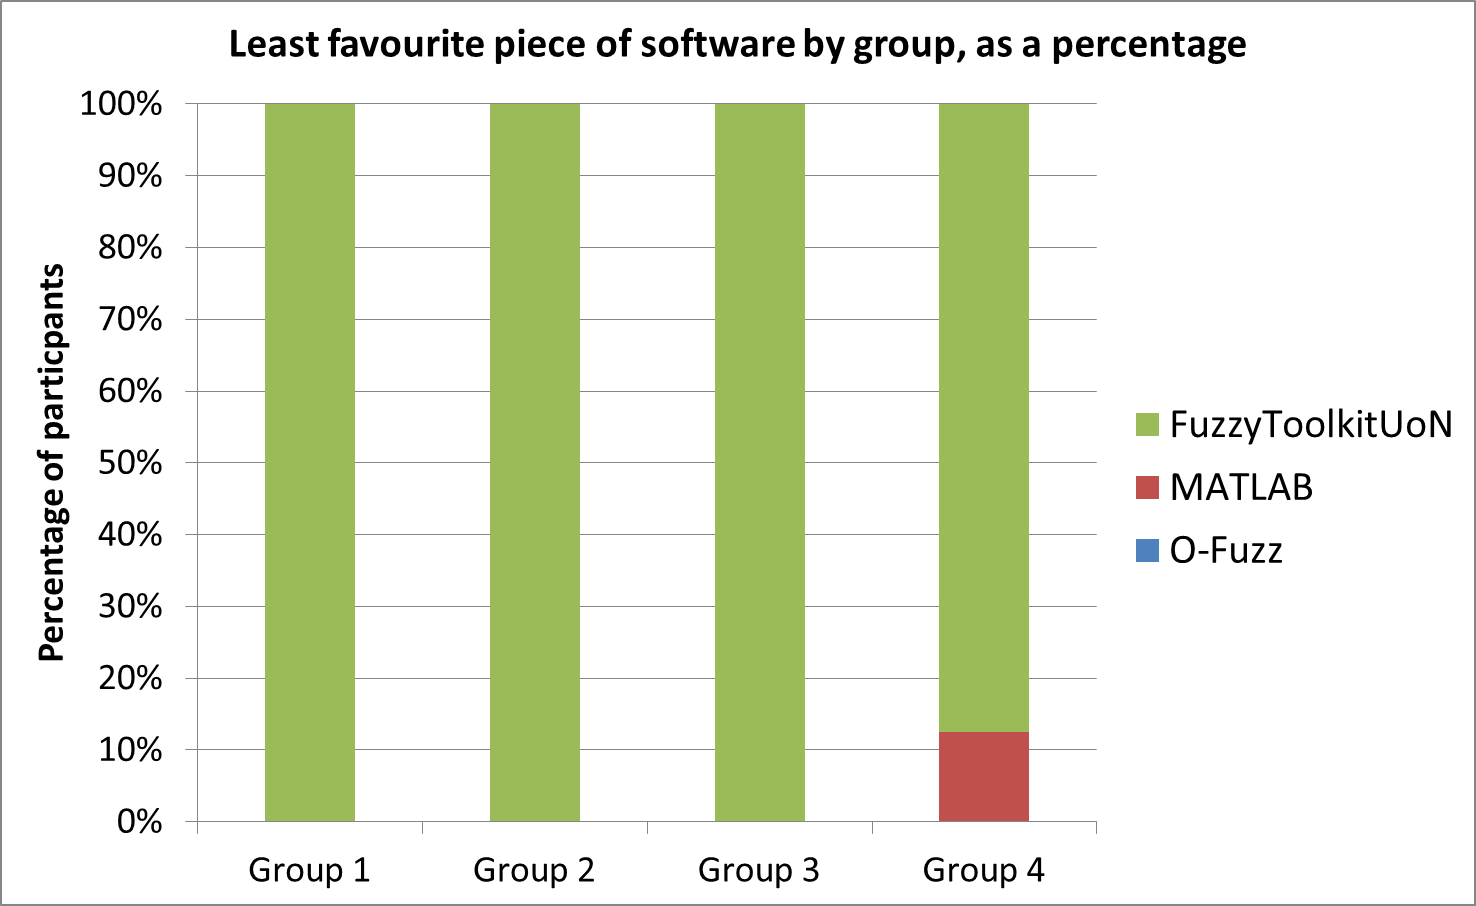
\includegraphics[width=0.65\textwidth]{images/leastFav}
	\end{center}
	\vspace{-5mm}
	\captionsetup{justification=centering,margin=2cm}	
	\caption{The percentage of users claiming each piece of software to by their least favourite}
	\label{fig:leastFavour}
	\vspace{-2mm}
\end{figure}
\noindent 
The piece of software that was most favoured by the test participants, was the system proposed in this report, o-Fuzz. Of the total participants, 65\% claimed o-Fuzz to be their favourite software, with 30\% saying it was MATLAB, and 4\% saying FuzzyToolkitUoN (a single person). A decomposition of favourite software across groups can be seen in figure \ref{fig:mostLiked}
			
\begin{figure}[ht!]
	\begin{center}
		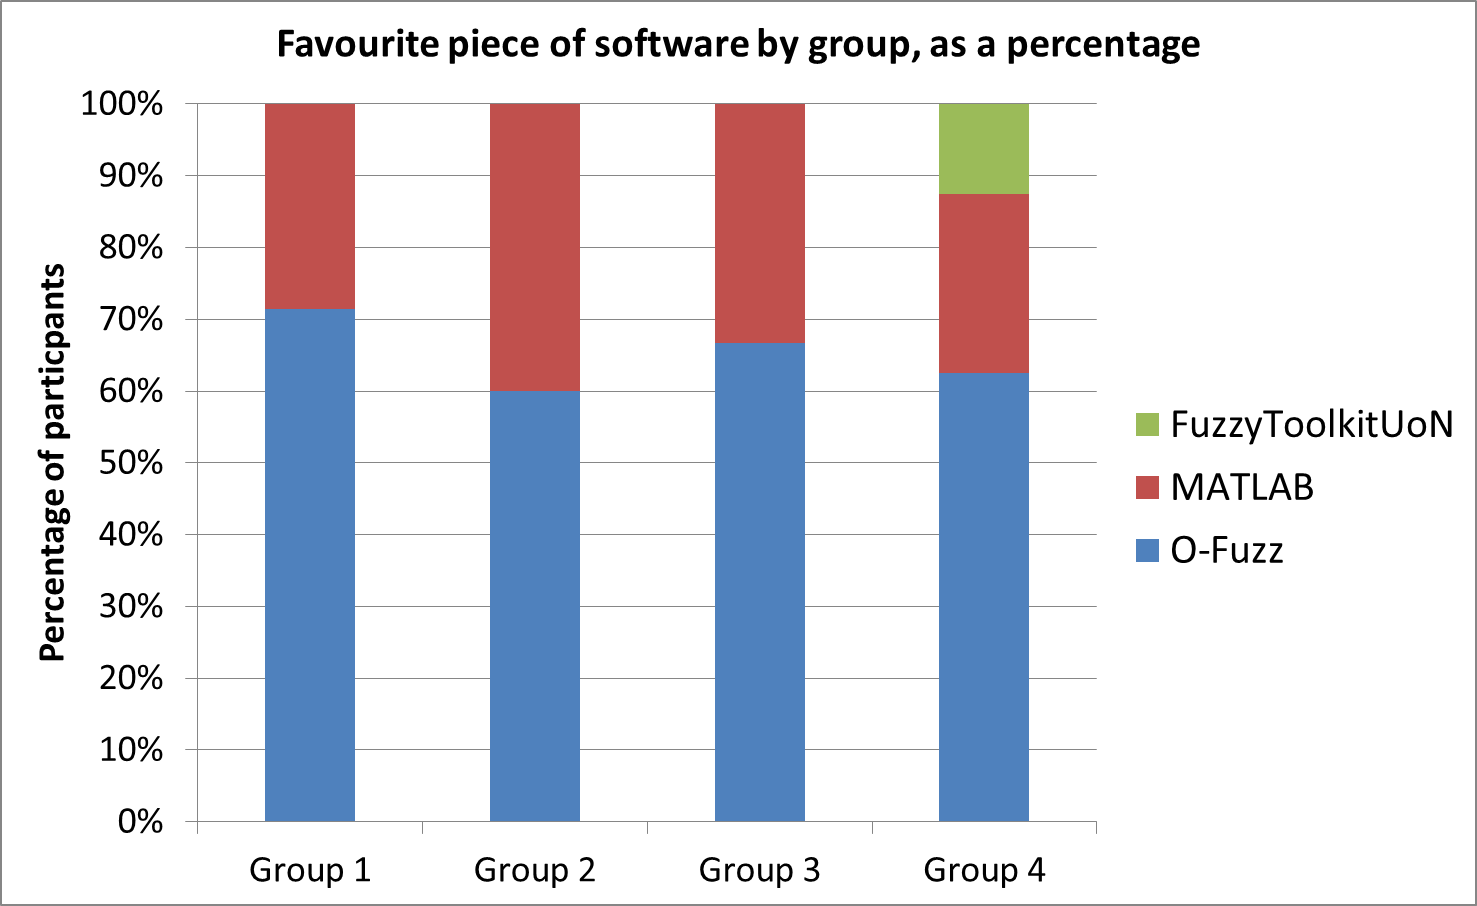
\includegraphics[width=0.65\textwidth]{images/mostFav.png}
	\end{center}
	\vspace{-5mm}
	\captionsetup{justification=centering,margin=2cm}	
	\caption{The percentage of users claiming each piece of software to by their most favourite}
	\label{fig:mostLiked}
	\vspace{-2mm}
\end{figure}
\noindent 
When questioned as to the preference of this new system, most users agreed that the interface was both extremely simple to navigate, and visually appealing. It was also mentioned that there was a natural flow to the software. By this, they meant that each task in the software lead onto the next very intuitively. For instance, the adding of a variable would be one distinct task, but the adding of membership functions would be a separate task nested inside this task. This meant that the conceptually distinct parts of the system were separate, but the system had a ``waterfall'' style flow to it. Many of the novice users also commended the system on it's help system, specifically mentioning how this was much more intuitive than checking the huge documentation manual provided with FuzzyToolkitUoN.\ \\
\ \\
It is worth noting that the single result for FuzzyToolkitUoN as favourite software came from a user that was extremely proficient in R, and specifically FuzzyToolkitUoN, and knew many commands from memory. 
	

\subsection{Successes and Limitations of the Project}
% Successes:
% Fulfills its main two goals
% Easy to pick up by a novice user 
% Easily expandable
% Deals with errors well

% Limitations
% Backend did not provide a lot of functionality -> Get new backend/API Layer
% Some other issue..
% Some other issue..